%!TEX root = ../main.tex
\subsection{CNN evaluation on human perception}
\label{sec:cnn-evaluation-perception}

\begin{figure}
\centering
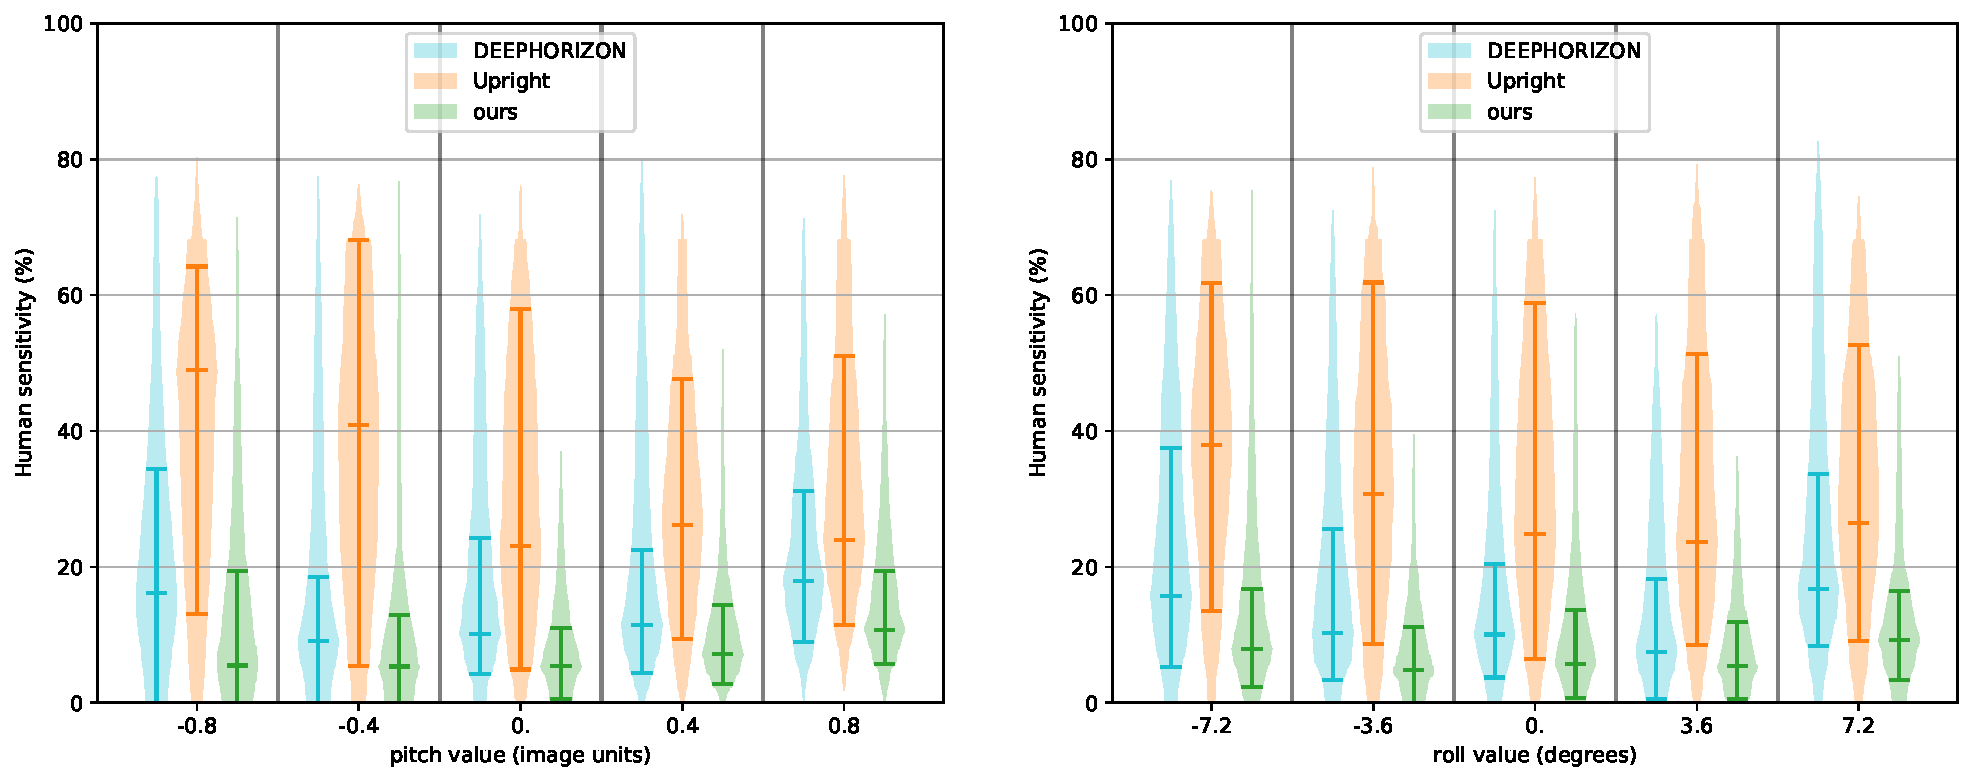
\includegraphics[width=\linewidth]{figures/method/human_sensitivity_performance_SUN360.pdf}
\begin{tabular}{p{0.5\linewidth}p{0.5\linewidth}}
\hspace{1.5cm}(a) & \hspace{1.3cm}(b)
\end{tabular}
\caption[Performance on human sensitivity measure]{Performance of our method, Upright and DEEPHORIZON on (a) pitch and (b) roll using our human sensitivity measure. Reported sensitivity takes into account estimation errors on all three parameters at the same time.}
\label{fig:method_human_performance}
\end{figure}


We further evaluate the method we proposed in sec.~\ref{sec:proposed_method} against other learning and non-learning-based methods in terms of the human sensitivity. To obtain a human sensitivity function, we fit a kNN with k=15 to the human sensitivity study results of this section. Specifically, we use error and parameter values on pitch, roll and field of view, yielding a 6 degrees of freedom function. We use the Euclidean distance for neighbor selection and scaled each value according to observed tolerance in the user study: $1{:}0.2$ for pitch in image units, $1{:}12$ for roll in angle and $1{:}15$ for field of view in angle. We convert the reported percentage of human choosing the ground truth values to human sensitivity by mapping the 50-100\% range (confusion-detection) to 0-100\%. Performance on this human sensitivity function on our SUN360 test set for horizon estimation is shown in fig.~\ref{fig:method_human_performance}. Our method has the third quartile of its predictions under 20\% of human sensitivity across the parameter range, systematically lower than every other method. Even though our method was not directly trained using a perceptual loss, we believe this improvement is due to the entropy-based loss being stricter than the perceptual loss (i.e., it penalizes all errors even when they don't affect the realism).

To further assess the perceived accuracy of our method, we ran another user study that showed participants object insertion results using 3 calibration methods simultaneously and asked them to pick the most realistic one. Table~\ref{tab:user_comparison} shows the scores from 2208 votes (32 users $\times$ 69 images).

\begin{table}[!h]
\centering
%\footnotesize
\vspace{-0.5em}
\begin{tabular}{lll}
\toprule
ours & \cite{Workman2016} & \cite{Lee2014} \\
\midrule
46\% & 31\% & 23\% \\
\bottomrule
\end{tabular}
\vspace{0.5em}
\caption[Human method preference study results]{User study comparing human preference on virtual object insertion. Percentage represents each method share of votes.}
\label{tab:user_comparison}
\end{table}
